\subsection{So sánh AI với luật ngưỡng và kiểm tra độ nhạy}
Lượt đánh giá bổ sung dùng nguyên \code{ai/model.joblib}, không ghi đè model. Module lưu hash model/CSV, kiểm tra 1.200 dự đoán gốc khớp toàn bộ file đã lưu và xuất từng mẫu vào \code{evidence/ai_evaluation_trials.csv}. Các mẫu mà ít nhất một phương pháp dự đoán sai nằm trong \code{evidence/ai_error_samples.csv}. Kết quả tổng hợp ở \code{evidence/ai_evaluation.json}.

Baseline là luật từng mẫu $T\geq32$~°C hoặc $RH\geq80$\%, không có trạng thái hysteresis. Nhãn bộ test đến từ thành phần bộ sinh normal/hot/humid chứ không được tính bằng luật này. Năm seed 26101--26105 tạo thêm 6.000 mẫu cùng phân bố; model và ngưỡng đều cố định trước đánh giá. Đây chỉ kiểm tra thay đổi mẫu ngẫu nhiên, chưa kiểm tra nhiều model huấn luyện hoặc tính tổng quát trên phòng thật.

\begingroup\small
\begin{longtable}{P{3.9cm}P{2.7cm}r r r r}
\caption{Model cố định so với luật ngưỡng; toàn bộ là dữ liệu sinh}\label{tab:ai-comparison}\\
\toprule Tập đánh giá & Phương pháp & Acc. (\%) & Recall (\%) & FPR (\%) & F1 \\ \midrule
\endfirsthead
\toprule Tập đánh giá & Phương pháp & Acc. (\%) & Recall (\%) & FPR (\%) & F1 \\ \midrule
\endhead
Gốc, 1.200 mẫu & Isolation Forest & 98.58 & 99.25 & 1.75 & 0.9790 \\
Gốc, 1.200 mẫu & Ngưỡng 32/80 & 99.67 & 99.00 & 0.00 & 0.9950 \\
Năm seed mới, 6.000 mẫu & Isolation Forest & 98.30 & 97.80 & 1.45 & 0.9746 \\
Năm seed mới, 6.000 mẫu & Ngưỡng 32/80 & 99.88 & 99.65 & 0.00 & 0.9982 \\
Bất thường hiếm, 2.040 mẫu & Isolation Forest & 98.68 & 100.00 & 1.35 & 0.7477 \\
Bất thường hiếm, 2.040 mẫu & Ngưỡng 32/80 & 99.95 & 100.00 & 0.05 & 0.9877 \\
Normal dịch phân bố, 1.000 mẫu & Isolation Forest & 79.90 & --- & 20.10 & --- \\
Normal dịch phân bố, 1.000 mẫu & Ngưỡng 32/80 & 99.00 & --- & 1.00 & --- \\
Lạnh bất thường, 300 mẫu & Isolation Forest & 100.00 & 100.00 & --- & 1.0000 \\
Lạnh bất thường, 300 mẫu & Ngưỡng 32/80 & 0.00 & 0.00 & --- & 0.0000 \\
\bottomrule
\end{longtable}

\endgroup

FPR là $FP/(TN+FP)$, không phải số cảnh báo mỗi giờ. Dấu gạch thể hiện thiếu lớp tương ứng: tập normal dịch phân bố không có nhãn bất thường, tập lạnh không có nhãn normal. Không dùng recall/F1 trên tập chỉ có normal để xếp hạng phương pháp.

Trên bộ gốc, luật ngưỡng có accuracy 99,67\%, cao hơn AI 98,58\%; trên năm seed mới, luật đạt 99,88\%, AI đạt 98,30\%. Kết quả không ủng hộ tuyên bố AI tốt hơn luật cho tình huống nóng/ẩm đang mô phỏng. Bộ sinh tạo các cụm tách xa nhau nên luật cố định đã phù hợp; dự án giữ cả hai cơ chế và trình bày đúng ưu/nhược điểm.

\begin{figure}[H]\centering
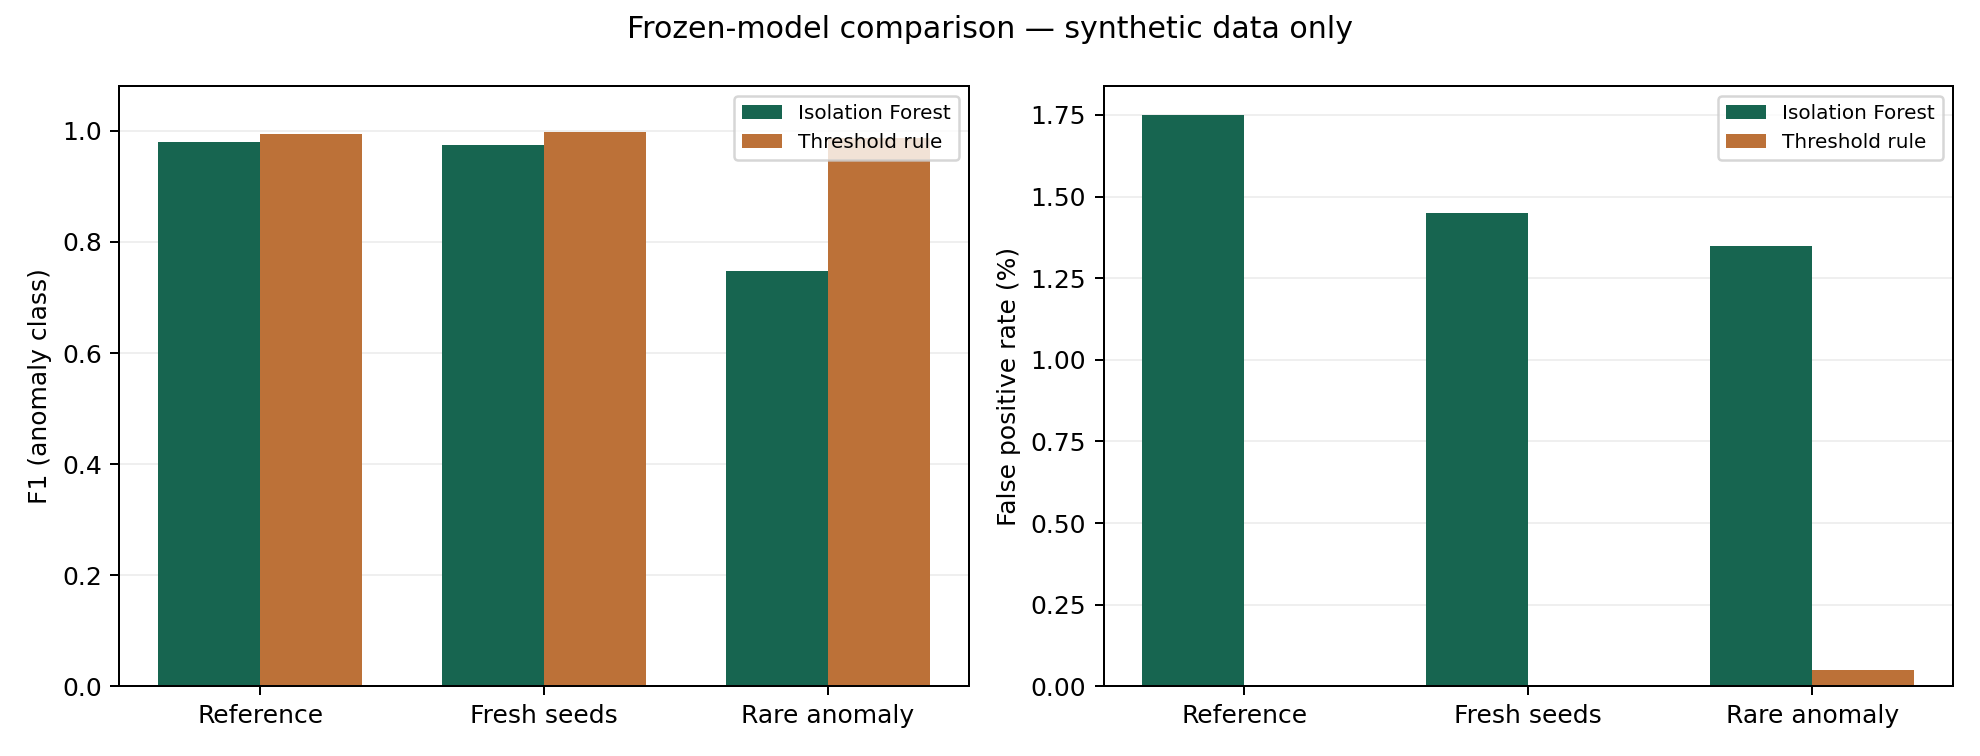
\includegraphics[width=\textwidth]{../evidence/ai_comparison.png}
\caption{F1 lớp bất thường và tỷ lệ báo động giả theo ba tập sinh; cùng một model và ngưỡng cố định.}
\end{figure}

\paragraph{Dịch phân bố normal.}
Một nghìn mẫu quanh 29~°C và 65\%RH, độ lệch chuẩn 1,3~°C/5\%RH, được kịch bản \emph{giả định} là normal. AI báo động giả \AIShiftFalseAlarm\%, so với 1,00\% của luật. Đây là thử độ nhạy với thay đổi điều kiện hợp lệ theo giả định, không phải nhãn đo ngoài thực địa. Model học quanh 27~°C/60\%RH có thể coi điều kiện mới là bất thường, vì vậy cần hiệu chỉnh bằng dữ liệu bối cảnh trước vận hành.

\paragraph{Bất thường hiếm.}
Tập 2.040 mẫu gồm 2.000 normal và 40 bất thường sinh; AI nhận đủ 40 nhưng báo sai thêm 27, nên precision chỉ \AIRarePrecision\% dù accuracy 98,68\%. Accuracy cao khi lớp normal chiếm đa số không đủ chứng minh cảnh báo đáng tin. Cần xem đồng thời TP/FP/FN, precision, recall và tần suất bất thường thực tế.

\paragraph{Lạnh chưa có trong tập train và các điểm sát biên.}
Ba trăm mẫu quanh 18~°C/40\%RH được bộ sinh đặt nhãn bất thường: AI phát hiện cả 300, luật chỉ có ngưỡng cao bỏ sót cả 300. Điều này minh họa phát hiện khác phân bố, không chứng minh AI vượt mọi luật; một luật thêm ngưỡng thấp cũng có thể xử lý tình huống này. Các điểm 32~°C, 80\%RH, 30~°C, 75\%RH và điểm dưới cả hai ngưỡng được kiểm tra qua gateway với model thật. Mỗi điểm dùng database mới để trạng thái hysteresis trước đó không ảnh hưởng đối chiếu. Đầu ra AI, score và inference time xuất hiện đúng trong payload chờ gửi cloud; lượt này không gửi dữ liệu thử lên tài khoản.

\begin{figure}[H]\centering
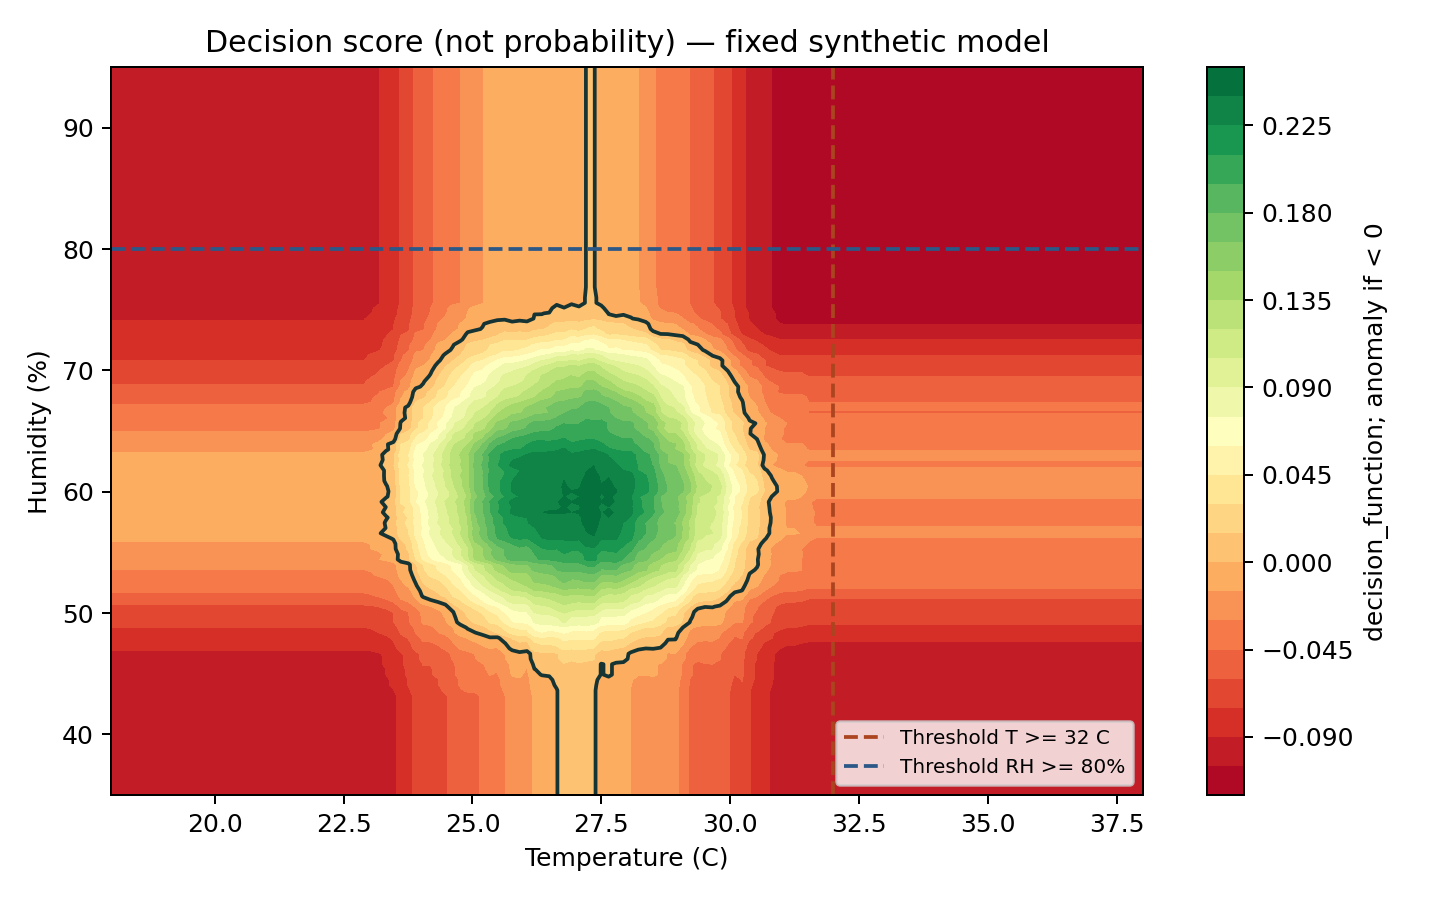
\includegraphics[width=.90\textwidth]{../evidence/ai_decision_regions.png}
\caption{Miền decision score của model cố định; đường score=0 tách nhãn AI, hai đường nét đứt là ngưỡng cao. Score không phải xác suất.}
\end{figure}

Sau 10 mẫu warm-up, đo 200 lần suy luận từng mẫu trên CPU có trung bình \AIExtendedMean~ms và P95 \AIExtendedPninetyFive~ms. Đây là lượt đo mới riêng ngày 26/11; không thay thế bảng benchmark đã lưu trước đó và không bao gồm đường truyền. Cả kiểm thử suy luận thật lẫn kiểm tra đầu vào CSV đều nằm trong bộ pytest hiện tại.
